\section{Vorgehensweise}

\subsection*{Projektplan}

\begin{figure}[h]
    \centering
    \begin{minipage}[b]{\textwidth}
        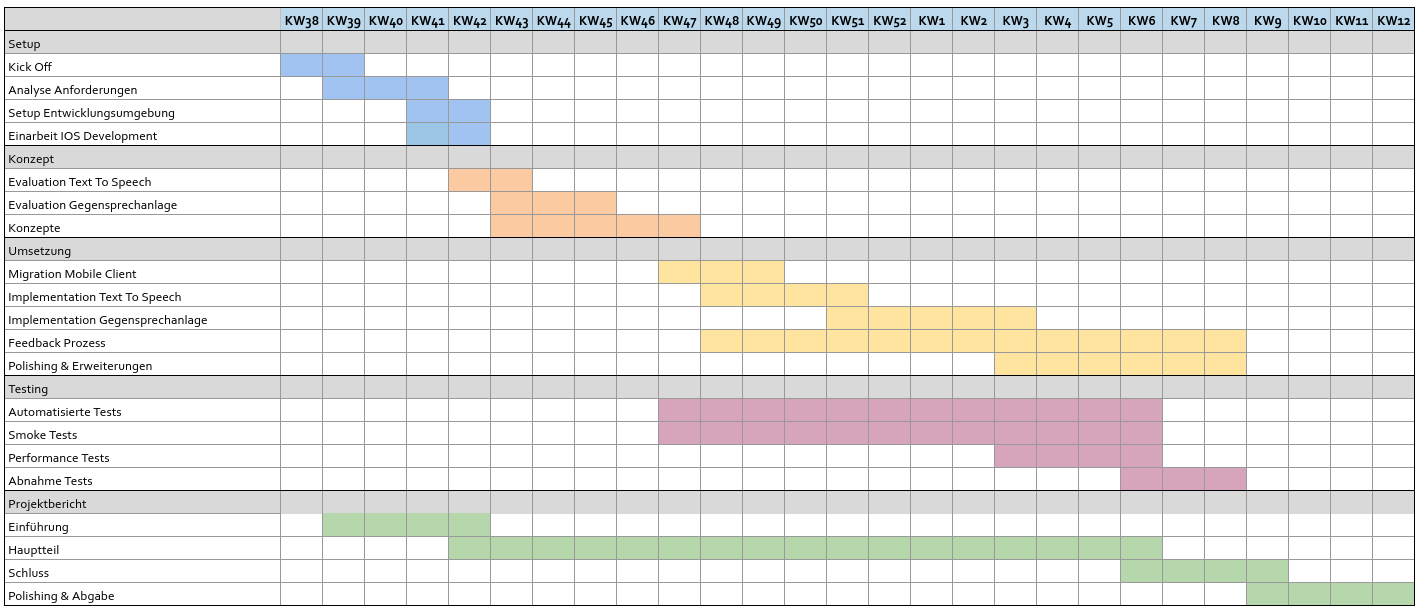
\includegraphics[width=\textwidth]{graphics/projektplan}
        \caption{Projektplan}
    \end{minipage}\label{fig:projektplan}
\end{figure}

Lorem ipsum
\clearpage

\subsection*{Meilensteine}

In der Anfangsphase des Projektes wurden folgende Meilensteine definiert:

\begin{table}[h]
    \centering
    \begin{tabular}{|l|p{15cm}|}
        \hline
        \textbf{Id} & \textbf{Beschreibung}                                                                                                                                                                                         \\
        \hline

        M01         & \textbf{Initiale Anforderungsanalyse}

        Die Anforderungen an das Projekt aus der Aufgabenstellungen sind in User Stories dokumentiert.\\
        \hline

        M02         & \textbf{Einarbeit und Setup IOS Umgebung}

        Projektteilnehmende sind mit groben Konzepten der IOS Entwicklung vertraut.
        Die Entwicklungsumgebung ist bereit für die Umsetzung. \\
        \hline

        M03         & \textbf{Evaluation Technologien}

        Die Evaluation der Technologien für Text To Speech und Gegensprechanalge (VOIP Kommuniation) ist abgeschlossen. \\
        \hline

        M04         & \textbf{Konzepte}

        Die Konzepte für Systemarchitektur, Aufbau und Architektur der mobilen Applikation sowie Anpassungen
        an bestehenden Kompenenten im System sind abgeschlossen. \\
        \hline

        M05         & \textbf{Migration betehender Funktionalität}

        Die Funktionen die im Mobile Client der Projektarbeit IP5 Cloudbasiertes Praxisrufsystem umgesetzt wurden,
        stehen in der neu entwickelten nativen IOS Applikation zur Verfügung. \\
        \hline

        M06         & \textbf{Umsetzung Text To Speech}

        Alle Anforderungen zu der Text To Speech Funktion sind in der neu entwickelten nativen IOS Applikation umgesetzt. \\
        \hline

        M07         & \textbf{Umsetzung Gegensprechanlage 1:1}

        Alle Anforderungen für die 1:1 Kommunikation über die Funktion Gegensprechanlage sind in der neu entwickelten nativen IOS Applikation umgesetzt. \\
        \hline

        M08         & \textbf{Umsetzung Gegensprechanlage 1:n}
        Alle Anforderungen für die 1:1 Kommunikation über die Funktion Gegensprechanlage sind in der neu entwickelten nativen IOS Applikation umgesetzt. \\
        \hline

        M09         & \textbf{Abnahme}

        Die Abnahmetests wurden zusammen mit dem Kunden ausgeführt. \\
        \hline



    \end{tabular}\label{tab:milestones}
\end{table}

\clearpage
